\chapter{Umsetzung und Implementierung}

In diesem Kapitel wird beschrieben, wie die neuronalen Netze, die für die Schüttgutprädiktion verwendet werden sollen,
umgesetzt und implementiert wurden.
Dafür wird auf die verwendete Software eingegangen und die Struktur der finalen Implementierung anhand eines Flussdiagramms betrachtet.
Am Ende des Kapitels wird ein genauerer Blick auf die verwendeten Hyperparameter und deren Optimierung geworfen.

% \todo[inline]{Sinnvoller einstiegstext in das Kapitel}


\section{Software}

% \color{blue}
% \begin{itemize}
%     \item Virtual Python environment.
%     \item Implementiert in TensorFlow. (angefangen in version 1.8, später nach 1.11 upgedatet)
%     \item tensorflow-gpu - .
%     \item Datenhandling: mit Pandas. Da Data Science ein wichtiger Part der Arbeit war, sehr wichtig erwähnen
%     \item Matplotlib für Visualisierung (die meisten selbstgemachten grafiken hier in der Arbeit)
%     \item OpenCV für Bilderdinge in der Pipeline (wie oben erwähnt)
%     \item MATLAB, für Tracksort und die Ursprünglichen implementation der Vergleichsdinge für evaluationen 
% \end{itemize}
% \color{black}

Für die Umsetzung der neuronalen Netze wurde im Rahmen dieser Arbeit 
das Open Source Framework TensorFlow\footnote{https://www.tensorflow.org/} verwendet.
Es wurde die \texttt{tensorflow-gpu} Variante mittels pip in einer Python~3.6.5 virtuellen Umgebung installiert.
Zu Beginn der Arbeit wurde die zum damaligen Zeitpunkt aktuelle TensorFlow Version 1.8 installiert, die zu einem späteren Zeitpunkt durch die Version~1.11 ersetzt wurde.

Für den Umgang mit den Daten wurde die Python Library \textit{pandas} in der Version~0.23.1 genutzt.
Weitere wichtige Software, die verwendet wurde 
% sind \textit{pandas} in der Version~0.23.1, was für den Umgang mit den Daten genutzt wurde, und 
ist \textit{matplotlib} in der Version~3.0.0, mit dem die Visualisierung der Ergebnisse und die meisten Grafiken dieser Arbeit generiert wurden.
Des Weiteren wurde die Python Bindings von \textit{OpenCV} in der Version~3.4.1.15 für die Verarbeitung der aufgenommen Bilder verwendet. \\
Der existierende \textit{Multi-Target-Tracking}-Algorithmus ist in \textsc{Matlab} implementiert worden. 
Deshalb sind Teile des Projekts, die direkt darauf aufbauen ebenfalls in \textsc{Matlab} geschrieben.

% \todo[inline]{Aufpassen dass das nicht zu viel wird}

\section{Code-Struktur}

Die grundlegende Struktur des Codes, der für das Training verantwortlich ist, ist in Abbildung~\ref{fig:impl01} dargestellt.
Aus der Hyperparameter-Datei werden die Hyperparameter geladen und basierend darauf der TensorFlow Custom Estimator initialisiert.
Außerdem werden die Daten aus den entsprechenden CSV-Dateien geladen 
und daraus jeweils ein \textit{pandas DataFrame} mit den Feature-Label-Paaren des Trainingssets und des Testsets generiert.
In der Trainingssschleife wird dann ein Modell mit dem Trainingsset trainiert.
Dies resultiert in dem trainierten Modell, das nun für die Prädiktion genutzt werden kann.

\begin{figure}[p]
    \centering
    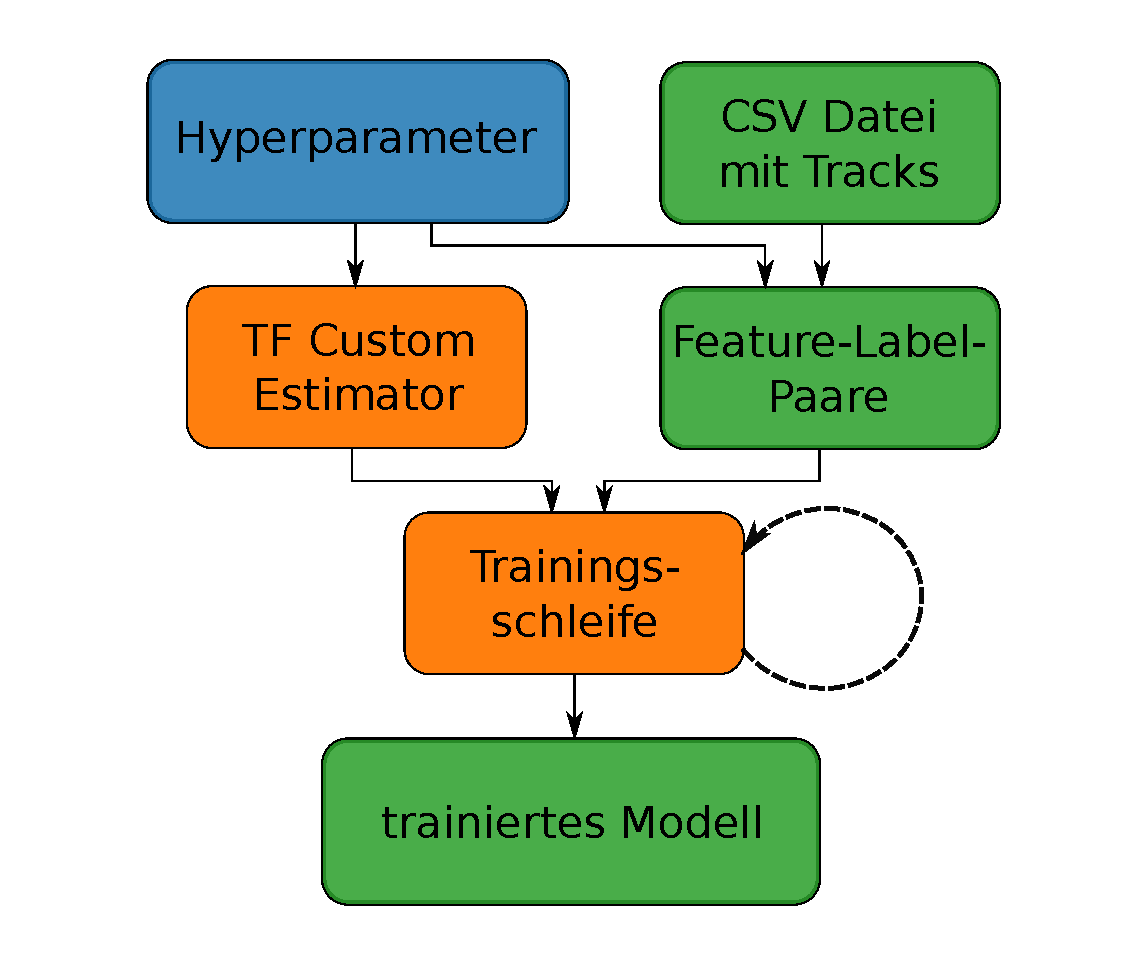
\includegraphics[width=0.75\textwidth]{implementation01v4.pdf}
    \caption{Skizzierter Trainingsablauf eines neuronalen Netzes}
    \label{fig:impl01}
\end{figure}


Der Ablauf der Evaluation ist in Abbildung~\ref{fig:impl02} dargestellt. 
Um das aus dem Training resultierende Modell auszuwerten, werden die Feature-Label-Paare des Testsets benutzt.
Dem Modell werden die Features als Eingabe gegeben, um die Prädiktionen des Netzes zu erhalten.
Am Ende steht als Ergebnis ein einzelnes \textit{pandas DataFrame} in dem alle Features, das zurücktransformierte Label, 
die Prädiktionen des Netzes und die Prädiktionen der verschiedenen Vergleichsmodelle jeweils für alle Feature-Label-Paare des Testsets enthalten sind.
Hinzu kommen noch die Fehler all dieser Prädiktionen, also die Differenz zwischen der Ground Truth, die im Label steht, und den Prädiktionen selbst.
Diese Fehler werden dann analysiert.
Es werden Durchschnitt, Median und Quartile gebildet, welche dann mittels Boxplots und Histogrammen visualisiert.
Diese Diagramme sind in Kapitel~\ref{cap:Eval} zu finden.

\todo[inline]{Tabelle mit inhalt von Dataframe?}

% \todo[inline]{überlegen wie viel ich überhaupt dazu schreiben soll - }

\begin{figure}[p]
    \centering
    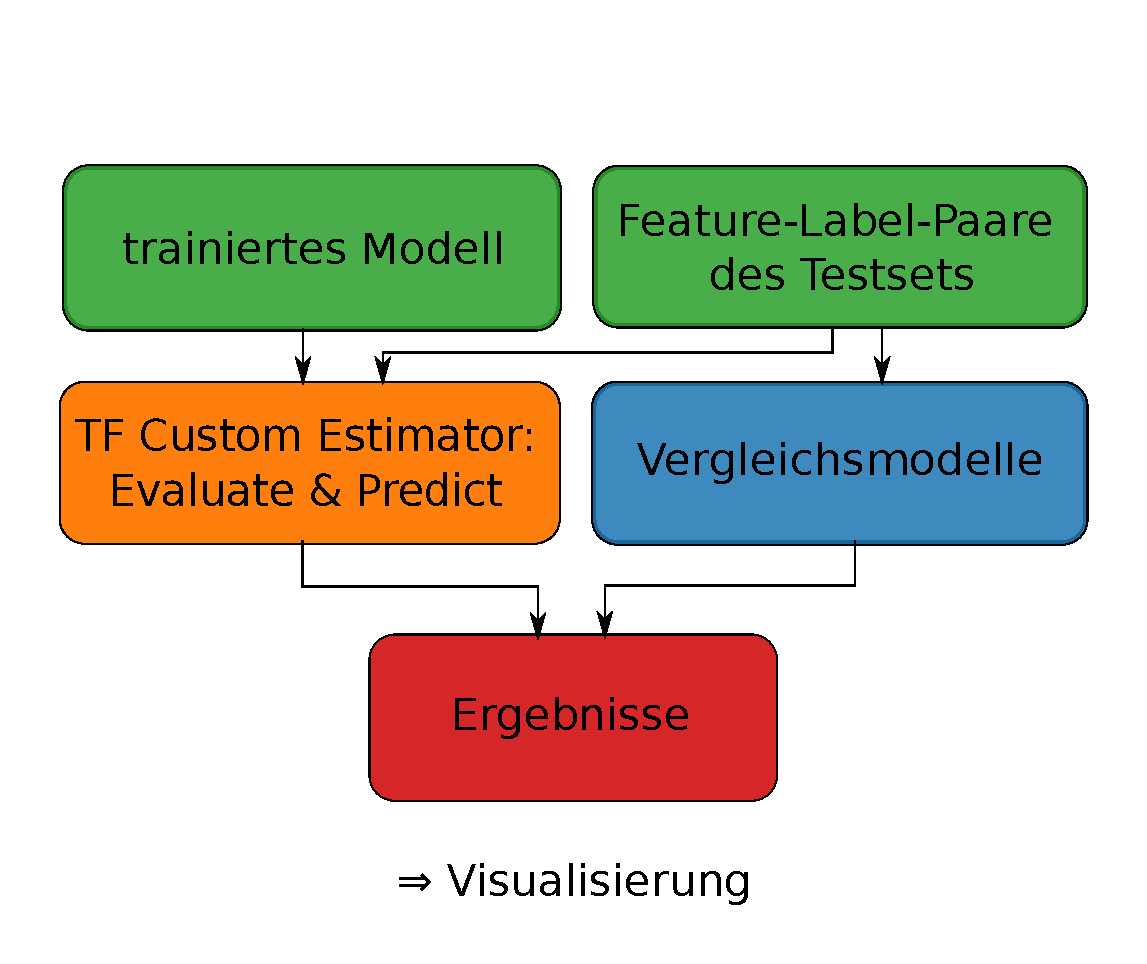
\includegraphics[width=0.75\textwidth]{implementation02v2.pdf}
    \caption{Skizzierte Ablauf der Auswertung des Ergebnis eines neuronalen Netzes}
    \label{fig:impl02}
\end{figure}


% \begin{figure}[h]
%     \centering
%     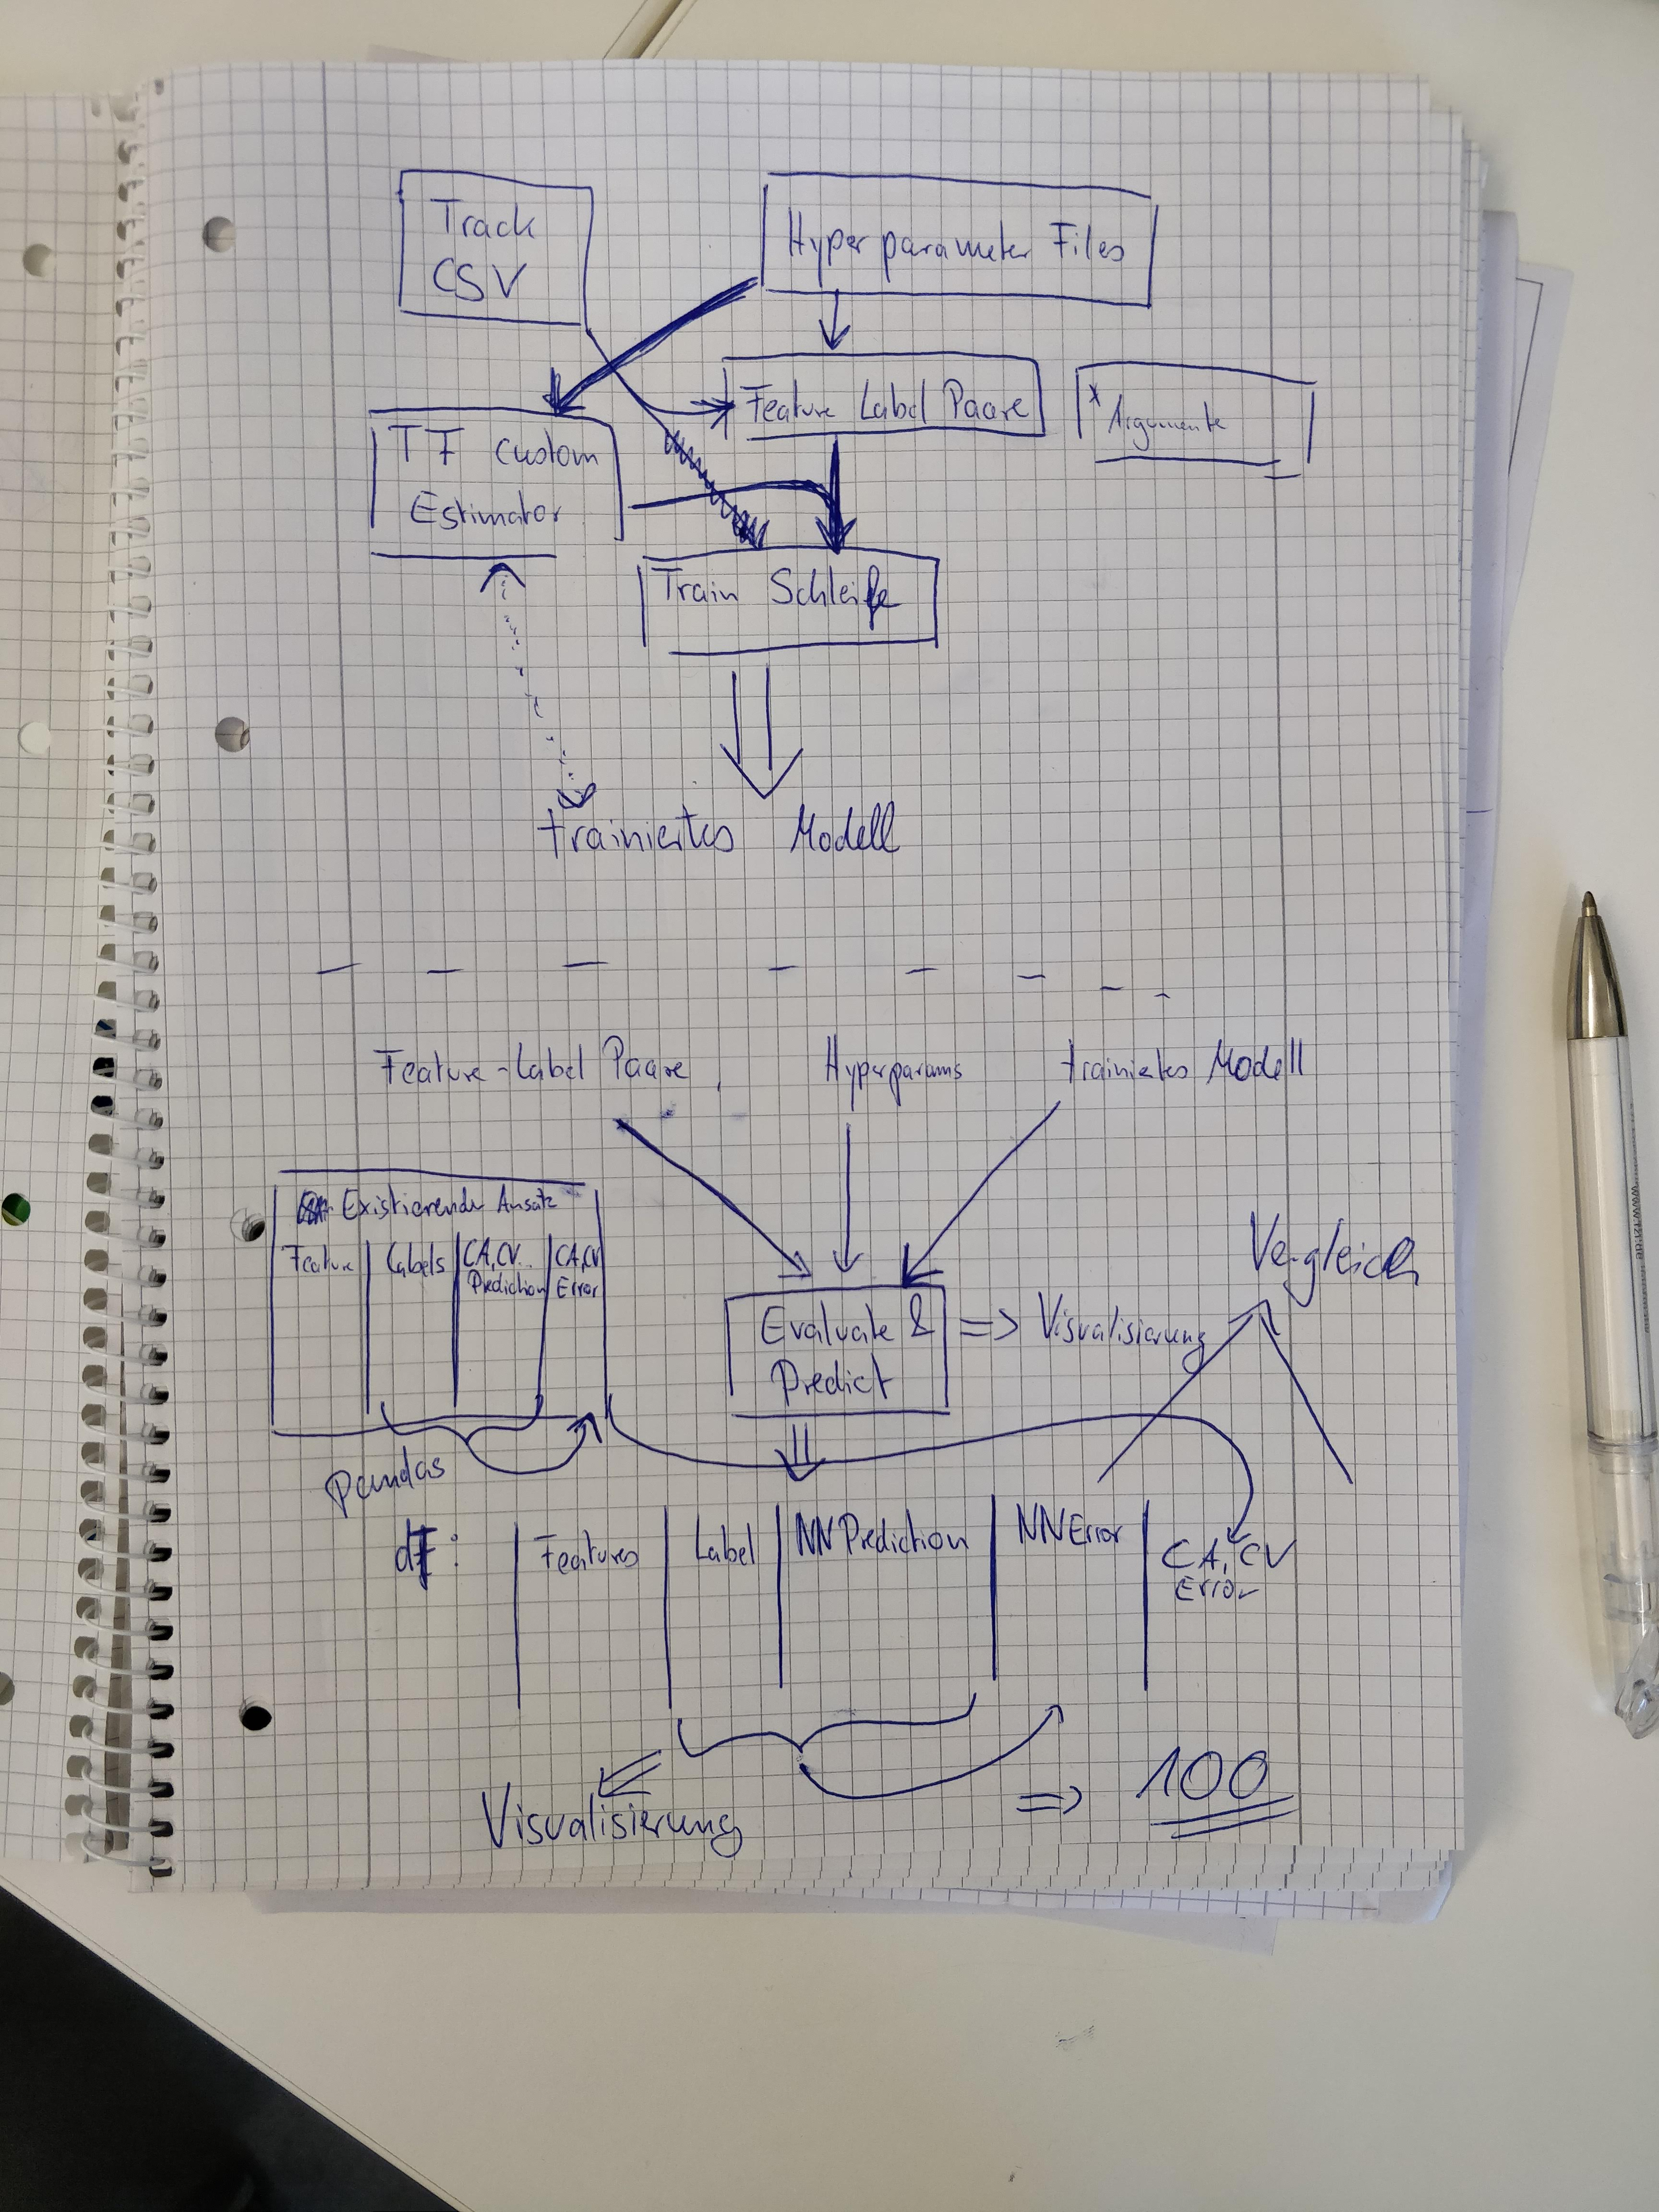
\includegraphics[width=\textwidth]{CodeStrukturSkizze}
%     \caption{Skizze Codestruktur}
%     \label{CodeStruktur}
% \end{figure}
  

\section{Hyperparameter}

% \color{blue}
% Hyperparameter sind die Variablen, die die Struktur des Netzes bestimmen (Eg: Anzahl Layers, FeatureSize) 
% sowie die Variablen, die festlegen wie das Netz trainiert (z.B. Lernrate, Anzahl Epochen)
% Hyperparameter werden vor dem Beginn des Trainings festgelegt und bleiben während dem kompletten Training unverändert.
% Vorgehen bei dieser Arbeit: Jeweils für NextStep und für Separator getrennte Konfigurationen finden.
% \color{black}

Im Kontext des maschinellen Lernens bezeichnet man jene Variablen als Hyperparameter, 
die bereits vor dem Beginn des Trainings festgelegt sein müssen.
Beispiele für solche Hyperparameter sind unter anderem Aspekte der Netzarchitektur, wie die Anzahl der Layers und ihre jeweilige Größe 
oder speziell im Falle dieser Arbeit die \textit{FeatureSize}, die festlegt welche Form der Input des Netzes annimmt.
Auch Parameter, die festlegen wie das Netz lernt - also Lernrate oder die Anzahl der Epochen beim Training - zählen dazu.

Bei der Implementierung dieser Arbeit wurde die Definition der Hyperparameter aus dem Programmcode selbst ausgelagert.
Stattdessen können sogenannte Hyperparameter-Dateien im JSON-Dateiformat definiert werden, die dann vom Programm geladen werden.
Dies vereinfacht das Training und das Evaluieren von Netzen mit unterschiedlichen Hyperparameter-Konfigurationen.
Einzelne Parameter aus den Dateien können per Kommandozeilenparameter überschrieben werden.
Ein Beispiel für eine solche Hyperparameter-Datei ist in Listing~\ref{lst-hyperparam} zu sehen.
Die Bedeutung der einzelnen Parameter soll im folgenden erklärt werden.

\todo[inline]{überlegen wir man das sinnvoll machen kann, dass das Listing seine eigene Seite kriegt und die Description sinnvoll anfängt.}

\newpage

\noindent\begin{minipage}{\textwidth}
\begin{lstlisting}[language=json,firstnumber=1, caption={Beispiel einer Hyperparameter-Datei in JSON}, captionpos=b, label=lst-hyperparam]

    {
        "arch": {
            "dropoutRate": 0.0,
            "hiddenLayers": [16, 16, 16],
            "featureSize": 5,
            "activation": "leaky_relu",
            "regularization": "no"
        },
        "problem": {
            "dataPath": "/home/hornberger/MasterarbeitTobias/data/selbstgesammelteDaten2/Kugeln-Band-Juli/",
            "modelBasePath": "/home/hornberger/MasterarbeitTobias/models/real/NextStep/NextStep-45kDecaySteps-SpheresReal",
            "imagePath": "/home/hornberger/MasterarbeitTobias/images/Real-NextStep-45kDecay-Spheres",
            "separator": 0,
            "separatorPosition": 1550,
            "thresholdPoint": 1200,
            "predictionCutOff": 1500

        },
        "train": {
            "batchSize": 500,
            "epochs": 3000,
            "stepsPerEpoch": 5000,
            "learningRate": 0.005,
            "decaySteps": 45000,
            "optimizer": "Adam"
        },
        "data": {
            "testSize": 0.1,
            "augmentMidpoint": 1123,
            "augmentRange": 1000,
            "direction": "x",
            "unitLoc": "px",
            "unitTime": "1/100 Frames",
            "limits": [0, 2350, 0, 1750]
        }
}

\end{lstlisting}
\end{minipage}
    
% \begin{itemize}
% \item Architektur:
%     \begin{itemize}
%         \item Dropout: Wahrscheinlichkeit für das zufälliges ausschalten von einzelnen Neuronen
%         \item Hidden Layer: ein Array an Zahlen repräsentiert die Architektur der Hidden Layers. Jede Zahl ist ein FC Layer mit so vielen neuronen
%         \item FeatureSize: Wie viele Positionen bekommt das Netz als Input ( \textrightarrow{} Größe des Inputlayers = 2x FeatureSize)
%         \item Activation: Aktivierungsfunktionen für die neuronen der Hidden Layers
%         % - optionen: "relu", "leaky_relu", "linear"
%     \end{itemize}
% \item Problem:
%     \begin{itemize}
%         \item DataPath: wo liegen die CSV Dateien zum die Daten rausladen
%         \item ModelPath: wo soll das Netz hingespeichert werden/Hergeladen - mit Checkpoints usw.
%         \item ImagePath: wo sollen Bilder hingespeichert werden, z.B. von Plot
%         \item separator: 0 oder 1, jenachdem ob es den nächsten Schritt (0) oder zum Düsenbalken (1) prädizieren soll
%     \end{itemize}

%     Falls Separator 1:
%     \begin{itemize}
%         \item separationPosition: Koordinate des Düsenbalken und Ziel der Prädiktion
%         \item ThresholdCutoff \todo{verify}
%         \item predictionCutOff: Koordinate hinter der keine FeatureTupel mehr genommen werden
%     \end{itemize}
% \item Train:

% \end{itemize}

% \begin{description}[align=right]
%     \item [Kate] some detail
%     \item [Christina]some detail
%     \item [Laura]some detail
% \end{description}

% \begin{itemize}
    % \item Architektur:

\newpage
% \bigskip
{\Large \sffamily \textbf{arch}}
\begin{description}[leftmargin=!,labelwidth=\widthof{\bfseries separatorPosition}, labelindent=0.5cm]
    \item [dropoutRate] Wahrscheinlichkeit für das zufällige Ausschalten von einzelnen Neuronen beim Training, entsprechend der Beschreibung in Unterabschnitt~\ref{ssec:Regul}.
    \item [hiddenLayers] Ein ein­di­men­si­o­nales Array an Zahlen, das die Architektur der Hidden Layers repräsentiert. Jede Zahl steht für ein Fully-Connected Layer mit der entsprechenden Anzahl Neuronen.
    \item [featureSize] Anzahl der vergangenen Positionen, die das Netz als Eingabe bekommt.
    \item [activation] Legt die Aktivierungsfunktionen für die Neuronen der Hidden Layers fest. Valide Optionen sind ReLU, Leaky ReLU und lineare Aktivierungsfunktionen.
    % - optionen: "relu", "leaky_relu", "linear"
\end{description}

\bigskip
{\Large \sffamily \textbf{problem}}

\begin{description}[leftmargin=!,labelwidth=\widthof{\bfseries separatorPosition}, labelindent=0.5cm]
    \item[dataPath] Ort im Dateisystem, wo die CSV-Dateien mit den Track Informationen liegen.
    \item[modelBasePath] Ort im Dateisystem, an dem das Modell des Netzes und alle damit verbundenen Dateien gespeichert wird, beziehungsweise woher es geladen wird. 
    \item [imagePath] Ort im Dateisystem, wo Schaubilder, Visualisierungen oder Ähnliches gespeichert werden sollen.
    \item [separator] Hyperparameter, der festlegt, für welche Art von Aufgabe das Netz trainiert werden soll. Für NextStep Netze steht hier 0 und für Separator Netze 1.
\end{description}

% Falls Separator 1:
\begin{description}[leftmargin=!,labelwidth=\widthof{\bfseries separatorPosition}, labelindent=0.5cm]
    \item[separatorPosition] Koordinate des Düsenbalken und Ziel der Prädiktion entlang der Bewegungsrichtung des Förderbands.
    \item[thresholdPoint] Koordinate des Punkts, ab dem prädiziert wird.
    \item[predictionCutOff] Koordinate des Punkts, ab dem die Tracks beim Laden abgeschnitten werden.
\end{description}

\bigskip
{\Large \sffamily \textbf{train}}

\begin{description}[leftmargin=!,labelwidth=\widthof{\bfseries separatorPosition}, labelindent=0.5cm]
    \item[batchSize] Die Anzahl der Feature-Label-Paare, die in einer Iteration betrachtet werden.
    \item[epochs] Die Anzahl der Epochen, für die trainiert wird.
    \item[stepsPerEpoch] Die Anzahl der Iterationen, die in einer Epoche durchgeführt werden.  
    \item[learningRate] Anfängliche maximale Lernrate, mit der die Gewichte geändert werden
    \item[decaySteps] Parameter, der festlegt, wie schnell die maximale Lernrate reduziert wird. 
    \item[optimizer] Der Optimierer, der fürs Training verwendet wird.
\end{description}

\bigskip
{\Large \sffamily \textbf{data}}
% \item Data:
\begin{description}[leftmargin=!,labelwidth=\widthof{\bfseries separatorPosition}, labelindent=0.5cm]
    % \item[numberFakeLines] Anzahl der synthetischen Trainingsbeispiele, die generiert werden sollen.
    \item[testSize] Parameter, der die Aufteilung zwischen Trainings- und Testdaten festlegt. Ein Wert von 0.1 würde einen 90:10 Split Training zu Test bedeuten.  
    \item[augmentMidpoint] Koordinate der Spiegelachse, an der für die Data Augmentation gespiegelt wird.
    \item[augmentRange] Maximale Distanz eines Feature-Label-Paares zur Spiegelachse, bis wohin immer noch die Spiegelung angewendet werden soll. Feature-Label-Paare mit einem Element außerhalb des Bandes werden ignoriert.
    \item[direction] Bewegungsrichtung der Partikel. ``x'' bei simulierten und ``y'' bei selbst gesammelten Daten.
    \item[unitLoc] Einheit des Orts. ``m'' beziehungsweise Meter bei simulierten Daten, ``px'' beziehungsweise Pixel bei selbst gesammelten Daten.
    \item[unitTime] Einheit der Zeit. 
    \item[limits] Bereich, der in der Visualisierung dargestellt wird.\\ \([0.388, \, 0.788, \ 0, \, 0.18]\) bei simulierten Daten und \([0,\, 2350, \ 0, \, 1750]\) bei selbst gesammelten Daten.

\end{description}
% \end{itemize}



\subsection{Hyperparameter Tuning}

% \color{blue}
% Als Hyperparameter Optimierung oder auch Hyperparameter Tuning bezeicht man den Vorgang das am besten geeignete Set an 
% Hyperparametern für einen Lernalgorithmus zu finden.

% Vorgehen um optimale Hyperparameter zu finden: 
% Baseline wird (über den Daumen gepeilt).
% Training mehrere Modelle mit variierenden Werten für einen einzelnen Parameter, 
% während die restlichen Parameter unverändert bleiben.

% So viele modelle zu trainieren ist sehr zeitintensiv, deshalb:
% Suchen auf Simulierten Daten (Spheres) und dann auf allen Daten verwenden.

% Nicht optimal... Maybe ausblick?


% Aktueller Stand:
% NextStep: kein Overfitting gefunden \textrightarrow L1 und L2 Regularisierung haben keinen positiven Effekt.\\
% Adam Optimizer ist am besten. \todo{erklären was genau der Adam optimizer eigentlich macht} \\
% leaky\_relu reigns supreme. \\
% Learning Rate Decay ist eine gute Idee. (Höherer Wert \textrightarrow langsamerer Zerfall). \\
% FeatureSize 5 ist gut, weniger wird schlechter und Mehr ist auch schlechter geworden (potenziell weil weniger Beispiele?)
% Dropout macht es kaputt, also auf 0.0 setzen

% Separator: ?
% \color{black}

Als Hyperparameter Optimierung oder auch Hyperparameter Tuning bezeicht man den Vorgang, das am besten geeignete Set an 
Hyperparametern für einen Lernalgorithmus zu finden.

In Rahmen dieser Arbeit wurden die Hyperparameter für die verschiedenen Szenarien manuell angepasst und verglichen.
Da es zu zeitintensiv wäre, diesen Vorgang für jedes einzelne Szenario, bestehend auf dem verwendeten Schüttgut und Art der Aufgabe, durchzuführen,
wurde insgesamt nur zwei Sets an Hyperparametern gesucht.
Jeweils eines für NextStep Netze und eines für Separator Netze.
Diese wurden beiden auf dem DEM-Kugel-Datensatz optimiert und dann auf die anderen Datensätze angewendet.
Von dieser Betrachtung ausgenommen wurden Hyperparameter, die das Lernen nicht beeinflussen.
Dies sind die Parameter der Kategorien {\sffamily \textbf{problem}}, in der Dateipfade und Problemdefinitionen zu finden sind, 
und {\sffamily \textbf{data}}, in der unter anderem die relative Größe des Testdatensets festgelegt wird.


Für beide Arten von Netzen hat sich gezeigt, dass Dropout nicht nur keine Verbesserung mit sich bringt, sondern tatsächlich die Qualität der Ausgabe merklich reduziert.
Deshalb wurde für die letztendlich verwendete Trainingskonfiguration die Dropout Rate für alle Szenarien auf 0.0 gesetzt. 
Auch bezüglich der Aktivierungsfunktionen und der Optimierer unterscheiden sich die beiden Aufgaben nicht. 
In beiden Fällen haben sich Leaky ReLU und der Adam Optimizer als beste Option hervorgetan.
\todo[inline]{Sollte ich erklären was genau der Adam Optimizer eigentlich macht?}

Eine während des Trainings sinkende Lernrate hat einen positiven Einfluss auf die Güte der Ausgabe der Netze gezeigt. 
Es wurde eine Technik names \textit{exponential learning rate decay} eingesetzt,
die die Lernrate, die an den Optimierer übergeben wird, in Abhängigkeit der absolvierten Trainingsschritte reduziert.   
Die verwendete Lernrate entspricht dabei der folgenden Formel:
\begin{equation*}
	\text{aktuelle Lernrate} = \text{Basislernrate} \cdot \lambda ^{\frac{\text{globaler Trainingsschritt}}{\text{Zerfallsschritte}}}
\end{equation*}
Die Zerfallskonstante \(\lambda\) wurde als 0.96 festgelegt, während die Basislernrate und die Zerfallsschritte anpassbare Hyperparameter sind.


Das Ergebnis des Hyperparameter Tunings bezüglich Netzarchitektur für die NextStep Netze ist in Abbildung~\ref{fig:netArchitectureNextStep} zu sehen.
Auf den Testdaten produzierte von den erprobten Konfigurationen eine FeatureSize von 5 in Kombination mit 3 Hidden Layers mit jeweils 16 Neuronen die besten Ergebnisse.
Was die Lernparameter angeht, so sieht das Ergebnis des Hyperparameter Tunings folgendermaßen aus:
\begin{itemize}
    \item Batch Größe von 500
    \item Training über insgesamt 3000 Epochen mit jeweils 5000 Iterationen
    \item Basislernrate von 0.005 und 45\,000 Zerfallsschritte
\end{itemize}

\begin{figure}[h]
    \centering
    % \missingfigure{Grafik architektur}
	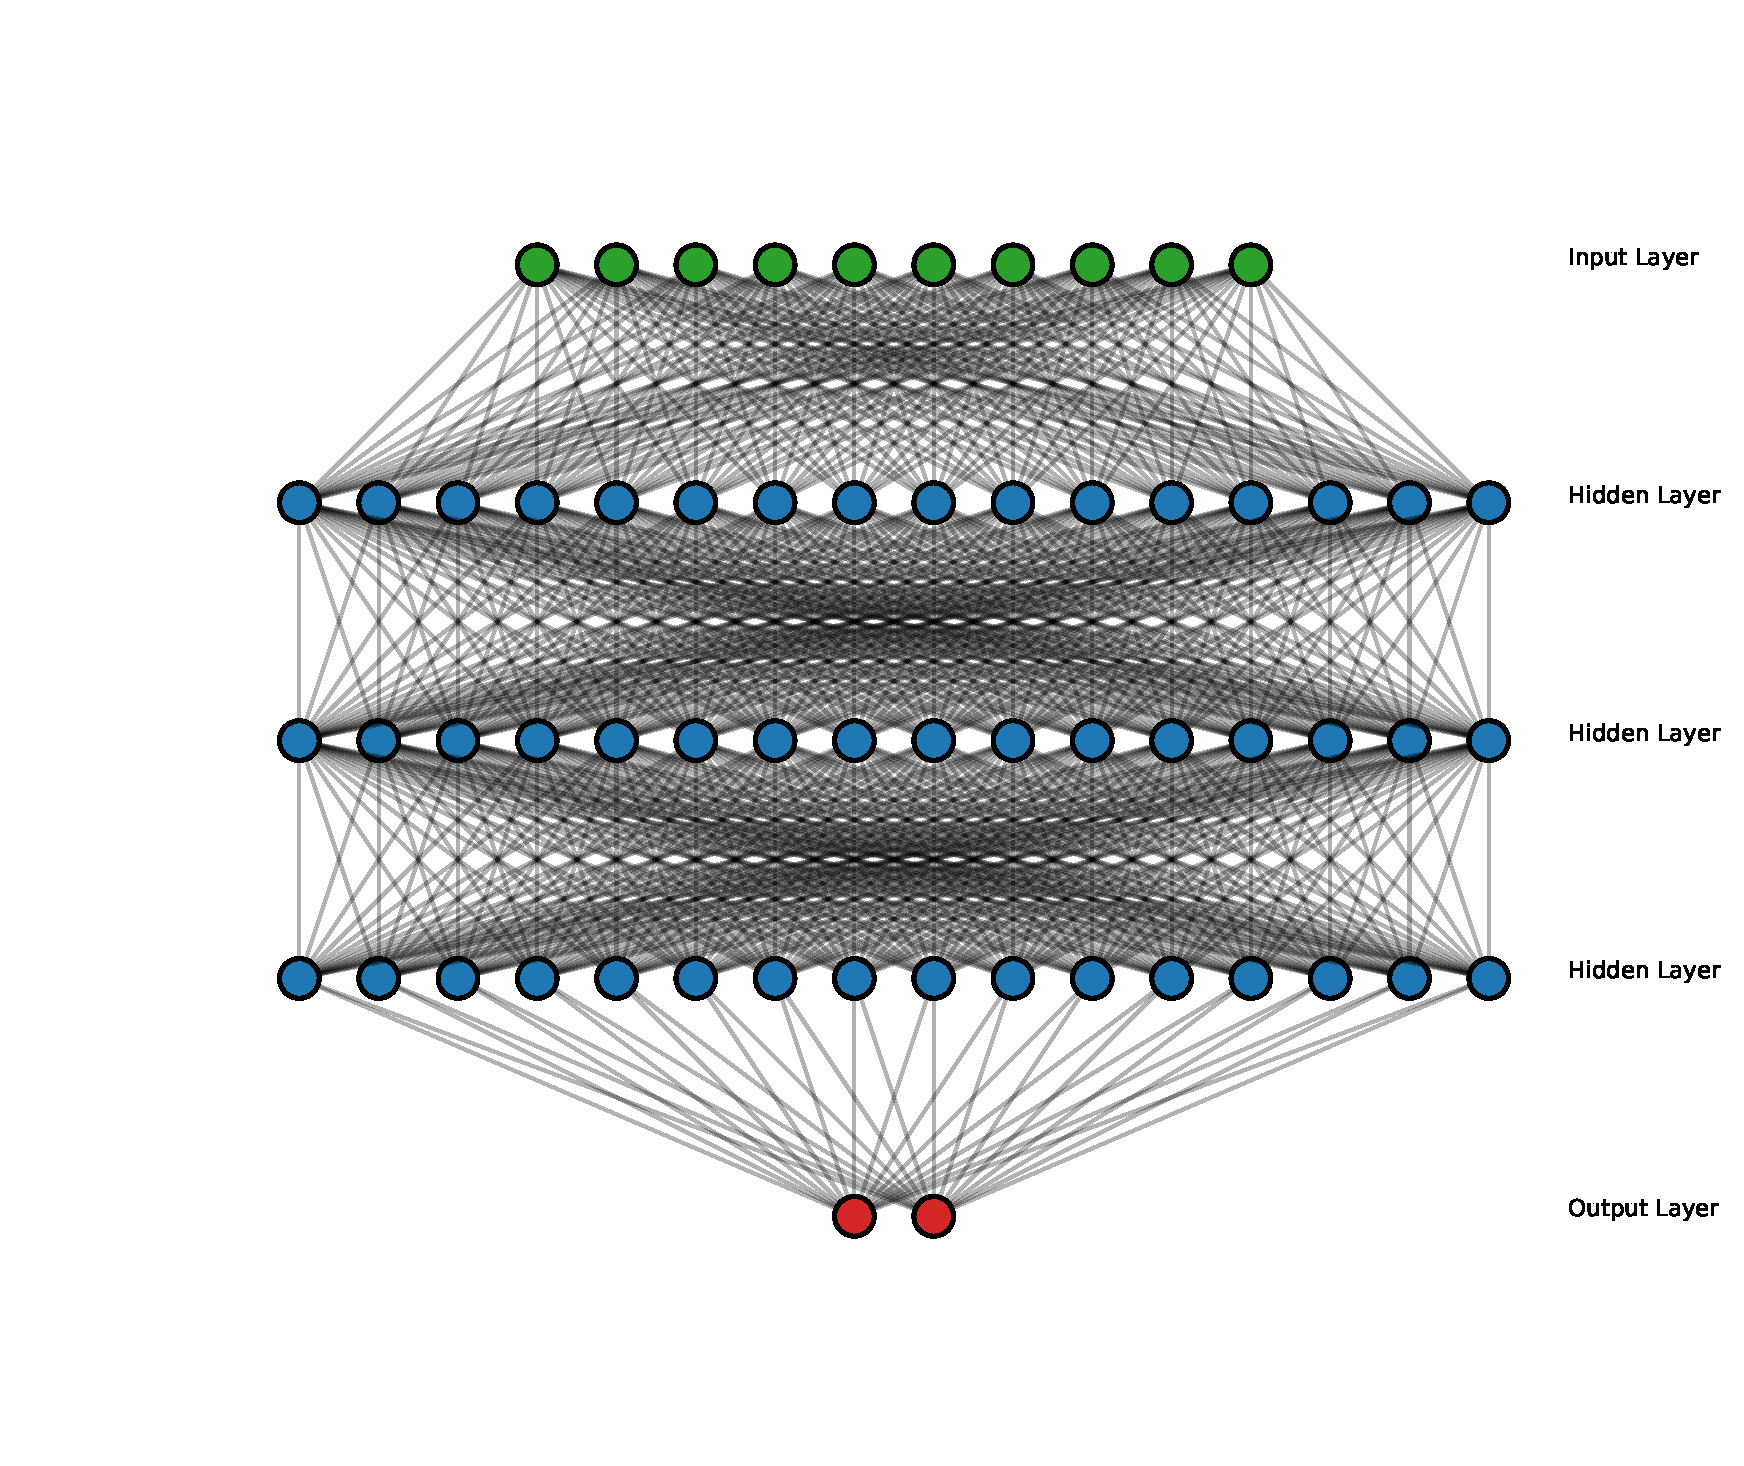
\includegraphics[width=\textwidth]{neuralNetImage}
	\caption{Architektur eines Neuronales Netzes für die NextStep Prädiktion}
	% \todo{Quelle Bild!}
	\label{fig:netArchitectureNextStep}
\end{figure}

Die Netzarchitektur, die für die Separator Netze  ermittelt wurde ist in Abbildung~\ref{fig:netArchitectureSep} zu sehen.
% \todo[inline]{Ergebnis von Hyperparameter Tuning für Separator Netze}\
Hier produzierte eine FeatureSize von 7 bessere Ergebnisse.
Dies erscheint plausibel, da für die Separator Netze im Gegensatz zu den NextStep Netzen eine höhere FeatureSize nicht mit einer Reduktion der Anzahl an Trainingsbeispielen einhergeht.
\todo{Sind hier solche Vermutungen angebracht?}
Des Weiteren haben 4 Layers mit jeweils 16 Neuronen die besten Ausgaben von den erprobten Konfigurationen erzielt.
Das Hyperparameter Tuning hat für die restlichen Hyperparameter die folgenden Werte ergeben:
\begin{itemize}
    \item Batch Größe von 100
    \item Training über insgesamt 1000 Epochen mit jeweils 5000 Iterationen
    \item Basislernrate von 0.005 und 60\,000 Zerfallsschritte
\end{itemize}

% \input{NeuralNet.pgf}

\begin{figure}[h]
    \centering
    % \missingfigure{Grafik architektur Separator}
	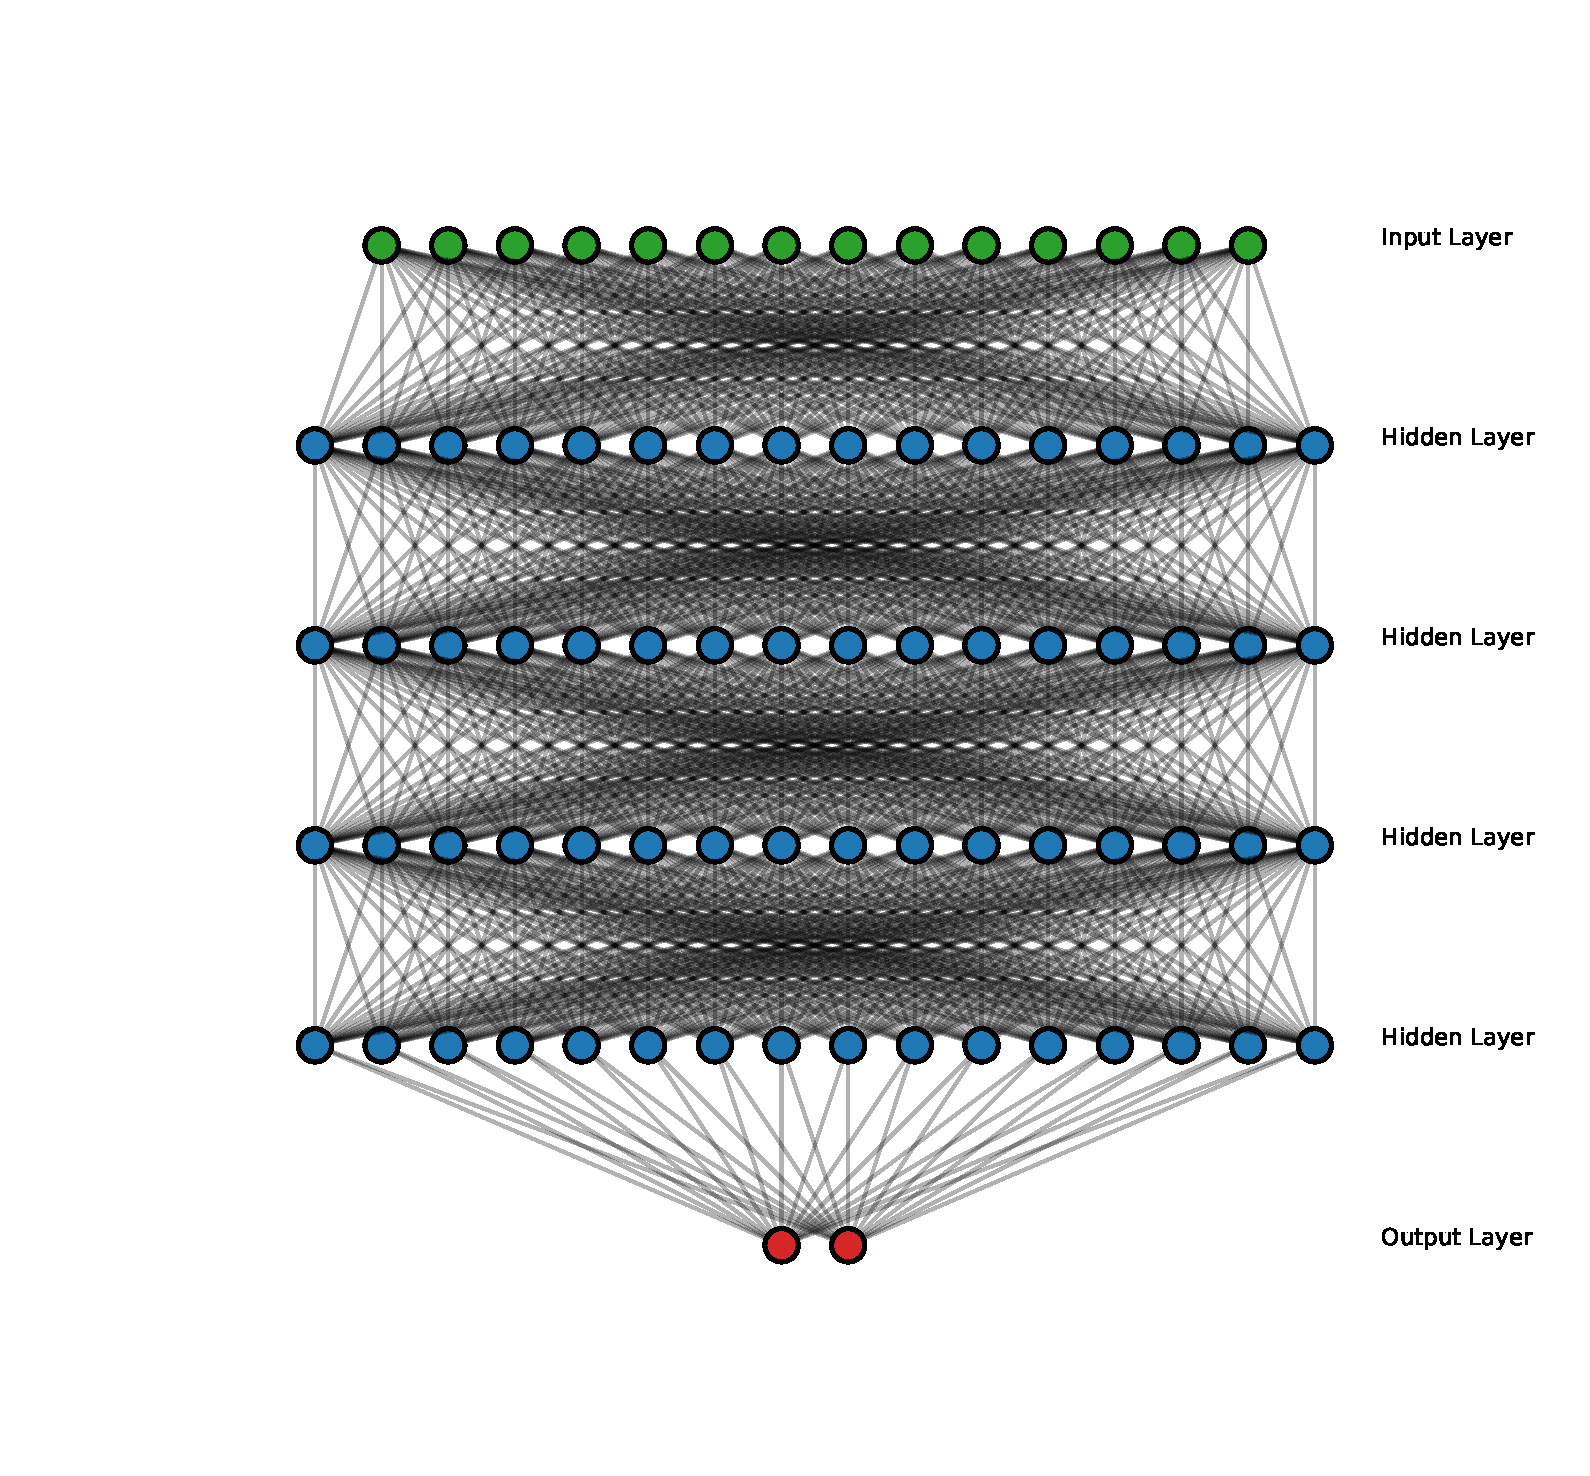
\includegraphics[width=\textwidth]{neuralNetImageSeparator}
	\caption{Architektur eines Neuronales Netzes für die Separator Prädiktion}
	% \todo{Quelle Bild!}
	\label{fig:netArchitectureSep}
\end{figure}


